\section*{Question 2}
Extending $\mathbf{P_1}$ and $\mathbf{P_2}$ to work on the full alphabet $\Sigma$ we get the non-deterministic finite automata seen in figure \ref{fig:P1P2}.

\vspace{1 cm}
\begin{figure}[H]
    \begin{center}
        \begin{tikzpicture}
        \offset = 7;
        
        %Process 1:
        \draw(0, 1) node [font = \large] {Process 1};
        
        %Initial state arrow
        \draw[very thick, ->] (-1,0) -- (-0.5,0);
        
        %State: q1
        \draw[color=black, thick](0,0) circle (0.5) node{$q_1$};
        
        %Edge from q1 to q1
        \draw[very thick, ->] (0.5,-0.3) .. controls (0.9,-0.2) and (0.9,0.2) .. (0.5,0.3);
        \draw(1.7, 0) node{$\mathrm{a_2, b_2, c_2}$};
        
        %Edge from q1 to q2
        \draw[very thick, ->] (0,-0.5) -- (0,-1.5);
        \draw(0.5, -1) node{$\mathrm{a_1}$};
        
        %State: q2
        \draw[color=black, thick](0,-2) circle (0.5) node{$q_2$};
        
        %Edge from q2 to q2
        \draw[very thick, ->] (0.5,-2.3) .. controls (0.9,-2.2) and (0.9, -1.8) .. (0.5, -1.7);
        \draw(1.7, -2) node{$\mathrm{a_2, b_2, c_2}$};
        
        %Edge from q2 to q3
        \draw[very thick, ->] (0,-2.5) -- (0,-3.5);
        \draw(0.5, -3) node{$\mathrm{b_1}$};
        
        %State: q3
        \draw[color=black, thick](0,-4) circle (0.5);
        \draw[color=black, thick](0,-4) circle (0.4) node{$q_3$};
        
        %Edge from q3 to q3
        \draw[very thick, ->] (0.5,-4.3) .. controls (0.9,-4.2) and (0.9, -3.8) .. (0.5, -3.7);
        \draw(1.7, -4) node{$\mathrm{a_2, b_2, c_2}$};
        
        %Edge from q3 to q1
        \draw[very thick, ->] (-0.5,-3.5) .. controls (-1.5,-2.5) and (-1.5,-1.5) .. (-0.5,-0.5);
        \draw(-1.8, -2.0) node{$\mathrm{c_1}$};
        
        
        
        %Process 2:
        \draw(\offset, 1) node [font = \large] {Process 2};
        
        %Initial state arrow
        \draw[very thick, ->] (-1+\offset,0) -- (-0.5+\offset,0);
        
        %State: q1
        \draw[color=black, thick](0+\offset,0) circle (0.5) node{$q_1$};
        
        %Edge from q1 to q1
        \draw[very thick, ->] (0.5+\offset,-0.3) .. controls (0.9+\offset,-0.2) and (0.9+\offset,0.2) .. (0.5+\offset,0.3);
        \draw(1.7+\offset, 0) node{$\mathrm{a_1, b_1, c_1}$};
        
        %Edge from q1 to q2
        \draw[very thick, ->] (0+\offset,-0.5) -- (0+\offset,-1.5);
        \draw(0.5+\offset, -1) node{$\mathrm{a_2}$};
        
        %State: q2
        \draw[color=black, thick](0+\offset,-2) circle (0.5) node{$q_2$};
        
        %Edge from q2 to q2
        \draw[very thick, ->] (0.5+\offset,-2.3) .. controls (0.9+\offset,-2.2) and (0.9+\offset, -1.8) .. (0.5+\offset, -1.7);
        \draw(1.7+\offset, -2) node{$\mathrm{a_1, b_1, c_1}$};
        
        %Edge from q2 to q3
        \draw[very thick, ->] (0+\offset,-2.5) -- (0+\offset,-3.5);
        \draw(0.5+\offset, -3) node{$\mathrm{b_2}$};
        
        %State: q3
        \draw[color=black, thick](0+\offset,-4) circle (0.5);
        \draw[color=black, thick](0+\offset,-4) circle (0.4) node{$q_3$};
        
        %Edge from q3 to q3
        \draw[very thick, ->] (0.5+\offset,-4.3) .. controls (0.9+\offset,-4.2) and (0.9+\offset, -3.8) .. (0.5+\offset, -3.7);
        \draw(1.7+\offset, -4) node{$\mathrm{a_1, b_1, c_1}$};
        
        %Edge from q3 to q1
        \draw[very thick, ->] (-0.5+\offset,-3.5) .. controls (-1.5+\offset,-2.5) and (-1.5+\offset,-1.5) .. (-0.5+\offset,-0.5);
        \draw(-1.8+\offset, -2.0) node{$\mathrm{c_2}$};
            
        \end{tikzpicture}
    \end{center}
    \caption{Extended versions of $\mathbf{P_1}$ and $\mathbf{P_2}$ working on the full alphabet $\Sigma$}
    \label{fig:P1P2}
\end{figure}

From these NFA’s we construct their intersection product $\mathbf{T}$. In order to make $\mathbf{T}$ deterministic, we add a state $D$ which acts as the dead state. All input symbols that would make either $\mathbf{P_1}$ or $\mathbf{P_2}$ stuck has an edge to $D$. $D$ has edges to itself for all symbols in the alphabet and is not a final state. 

The states in $\mathbf{T}$ will be shown as tuples of the respective states in the two NFA’s $\{q_{\mathbf{P_1}} , q_{\mathbf{P_2}} \}$. $\mathbf{T}$ can be represented with a transition function table calculated from the transition functions of $\mathbf{P_1}$ and $\mathbf{P_2}$. $\mathbf{T}$’s transition function is:
\begin{gather*}
    \delta_{\mathbf{T}}(\{q_{\mathbf{P_1}}, q_{\mathbf{P_2}}\}, \mathrm{a}) = \delta_\mathbf{P_1}(q_{\mathbf{P_1}}, \mathrm{a}) \cup \delta_\mathbf{P_2}(q_{\mathbf{P_2}}, \mathrm{a}) \\ 
    \hat{\delta}_{\mathbf{T}}(\{q_{\mathbf{P_1}}, q_{\mathbf{P_2}}\}, \mathrm{w}) = \hat{\delta}_\mathbf{P_1}(q_{\mathbf{P_1}}, \mathrm{w}) \cup \hat{\delta}_\mathbf{P_2}(q_{\mathbf{P_2}}, \mathrm{w})
\end{gather*} 
\quad for any symbol $\mathrm{a} \in \Sigma$, $\mathrm{w} \in \Sigma^*$ and states $\{q_{\mathbf{P_1}}, q_{\mathbf{P_2}}\}$, where $q_{\mathbf{P_1}} \in \mathbf{Q_{P_1}}$ and $q_{\mathbf{P_2}} \in \mathbf{Q_{P_2}}$. 

Using this, we can create the transition function table for $\mathbf{T}$ as seen in table \ref{tab:Tt}.

\begin{table}[H]
    \centering
    \begin{tabular}{|c||c|c|c|c|c|c|}
    \hline
    $\delta_{\mathbf{T}}$    & $\mathrm{a_1}$    &   $\mathrm{b_1}$   &    $\mathrm{c_1}$  &   $\mathrm{a_2}$   &   $\mathrm{b_2}$   &   $\mathrm{c_2}$ \\ \hline \hline
         
    $D$   & $D$     & $D$  & $D$    & $D$   & $D$   & $D$   \\ \hline
    
    $\rightarrow \{q_1, q_1\}$& $\{q_2, q_1\}$     & $D$  & $D$    & $\{q_1, q_2\}$   & $D$   & $D$   \\ \hline
    
    $\{q_1, q_2\}$  & $\{q_2, q_2\}$    & $D$   & $D$   & $D$   & $\{q_1, q_3\}$    & $D$   \\ \hline
   
    $\{q_1, q_3\}$  &   $\{q_2, q_3\}$  &   $D$ &   $D$ &   $D$ &   $D$ &   $\{q_1, q_1\}$  \\ \hline
   
    $\{q_2, q_1\}$  &   $D$ &   $\{q_3, q_1\}$  &   $D$ &   $\{q_2, q_2\}$  &   $D$ &   $D$ \\ \hline
   
    $\{q_2, q_2\}$  &   $D$ &   $\{q_3, q_2\}$  &   $D$ &   $D$ &   $\{q_2, q_3\}$  &   $D$ \\ \hline
   
    $\{q_2, q_3\}$  &   $D$ &   $\{q_3, q_3\}$  &   $D$ &   $D$ &   $D$ &   $\{q_2, q_1\}$  \\ \hline
   
    $\{q_3, q_1\}$  &   $D$ &   $D$ &   $\{q_1, q_1\}$  &   $\{q_3, q_2\}$  &   $D$ &   $D$ \\ \hline
   
    $\{q_3, q_2\}$  &   $D$ &   $D$ &   $\{q_1, q_2\}$  &   $D$ &   $\{q_3, q_3\}$  &   $D$ \\ \hline
    
    $*\{q_3, q_3\}$ &   $D$ &   $D$ &   $\{q_1, q_3\}$  &   $D$ &   $D$ &   $\{q_3, q_1\}$  \\ \hline
    
    
    \end{tabular}
    \caption{Transition functions for $\mathbf{T}$.}
    \label{tab:Tt}
\end{table}

As shown in table \ref{tab:Tt}, there are quite a lot of ways to end in state $D$, from where it is impossible to get to a final state. The final state for $\mathbf{T}$ is defined as:
\begin{gather*}
    F_{\mathbf{T}} = \{F_{\mathbf{P_1}}, F_{\mathbf{P_2}}\}
\end{gather*}
Meaning that the only final state for $\mathbf{T}$ is $\{q_3,q_3\}$. In the same manner, the initial state is given by a tuple of the initial states from $\mathbf{P_1}$ and $\mathbf{P_2}$, meaning that the initial state for $\mathbf{T}$ is $\{q_1, q_1\}$. 

The finite state machine for $\mathbf{T}$ is shown in figure \ref{fig:T}. The figure does not include all edges to the dead state $D$. All edges to $D$ can be seen in table \ref{tab:Tt}.

\begin{figure}[H]
    \begin{center}
        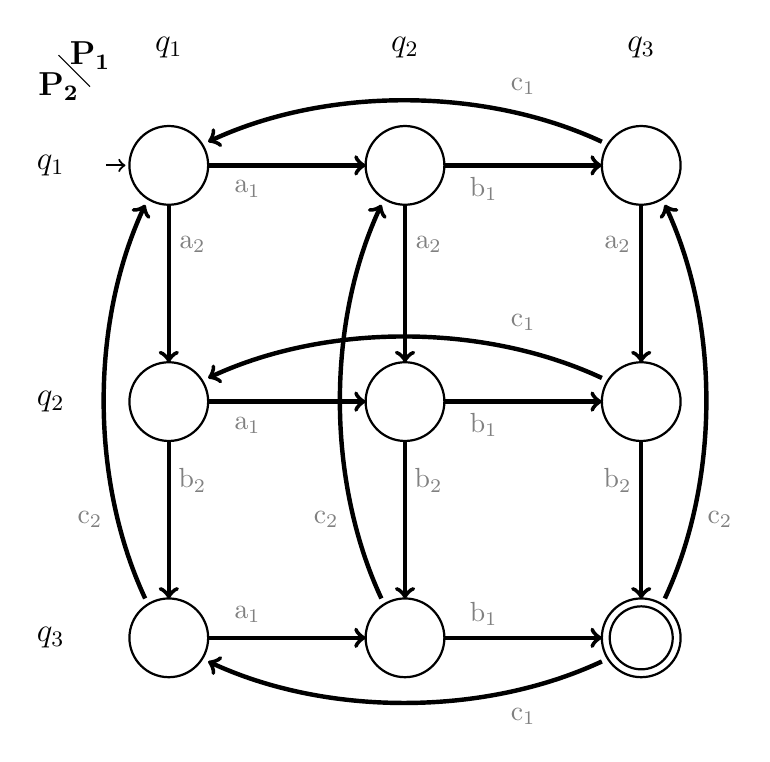
\begin{tikzpicture}
        %labels
        \draw(-1.0, 1.4) node [font = \large] {$\mathbf{P_1}$};
        \draw (-1.4, 1.4) -- (-1.0, 1.0);
        \draw(-1.4, 1.0) node [font = \large] {$\mathbf{P_2}$};
        
        \draw(0,1.5) node [font = \large] {$q_1$};
        \draw(3,1.5) node [font = \large] {$q_2$};
        \draw(6,1.5) node [font = \large] {$q_3$};
        
        \draw(-1.5,0)  node [font = \large] {$q_1$};
        \draw(-1.5,-3) node [font = \large] {$q_2$};
        \draw(-1.5,-6) node [font = \large] {$q_3$};
        
        %States
        \draw[thick, ->] (-0.8, 0) -- (-0.55, 0);
        \draw[color=black, thick](0,0) circle (0.5);
        \draw[color=black, thick](0,-3) circle (0.5);
        \draw[color=black, thick](0,-6) circle (0.5);
        \draw[color=black, thick](3,0) circle (0.5);
        \draw[color=black, thick](3,-3) circle (0.5);
        \draw[color=black, thick](3,-6) circle (0.5);
        \draw[color=black, thick](6,0) circle (0.5);
        \draw[color=black, thick](6,-3) circle (0.5);
        \draw[color=black, thick](6,-6) circle (0.5);
        \draw[color=black, thick](6,-6) circle (0.4);
        
        %Edges
            %horizontal 
            
        \draw[gray](4.5, 1) node {$\mathrm{c_1}$};
        \draw[color=black, ultra thick, <-] (0.5, 0.3) .. controls (2, 1) and (4, 1) .. (5.5, 0.3);
        
        \draw[gray](1, -0.3) node {$\mathrm{a_1}$};
        \draw[color=black, ultra thick, ->] (0.5, 0) -- (2.5, 0);
        
        \draw[gray](4, -0.3) node {$\mathrm{b_1}$};
        \draw[color=black, ultra thick, ->] (3.5, 0) -- (5.5, 0);
    
        
        \draw[gray](4.5, -2) node {$\mathrm{c_1}$};
        \draw[color=black, ultra thick, <-] (0.5, -2.7) .. controls (2, -2) and (4, -2) .. (5.5, -2.7);
        
        \draw[gray](1, -3.3) node {$\mathrm{a_1}$};
        \draw[color=black, ultra thick, ->] (0.5, -3) -- (2.5, -3);
        
        \draw[gray](4, -3.3) node {$\mathrm{b_1}$};
        \draw[color=black, ultra thick, ->] (3.5, -3) -- (5.5, -3);
        
        
        \draw[gray](4.5, -7) node {$\mathrm{c_1}$};
        \draw[color=black, ultra thick, <-] (0.5, -6.3) .. controls (2, -7) and (4, -7) .. (5.5, -6.3);
        
        \draw[gray](1, -5.7) node {$\mathrm{a_1}$};
        \draw[color=black, ultra thick, ->] (0.5, -6) -- (2.5, -6);
        
        \draw[gray](4, -5.7) node {$\mathrm{b_1}$};
        \draw[color=black, ultra thick, ->] (3.5, -6) -- (5.5, -6);
        
        
            %vertical
            
        \draw[gray](-1, -4.5) node {$\mathrm{c_2}$};
        \draw[color=black, ultra thick, <-] (-0.3, -0.5) .. controls (-1, -2) and (-1, -4) .. (-0.3, -5.5);
        
        \draw[gray](0.3, -1) node {$\mathrm{a_2}$};
        \draw[color=black, ultra thick, ->] (0, -0.5) -- (0, -2.5);
        
        \draw[gray](0.3, -4) node {$\mathrm{b_2}$};
        \draw[color=black, ultra thick, ->] (0, -3.5) -- (0, -5.5);
        
        
        \draw[gray](2, -4.5) node {$\mathrm{c_2}$};
        \draw[color=black, ultra thick, <-] (2.7, -0.5) .. controls (2, -2) and (2, -4) .. (2.7, -5.5);
        
        \draw[gray](3.3, -1) node {$\mathrm{a_2}$};
        \draw[color=black, ultra thick, ->] (3, -0.5) -- (3, -2.5);
        
        \draw[gray](3.3, -4) node {$\mathrm{b_2}$};
        \draw[color=black, ultra thick, ->] (3, -3.5) -- (3, -5.5);
        
        
        \draw[gray](7, -4.5) node {$\mathrm{c_2}$};
        \draw[color=black, ultra thick, <-] (6.3, -0.5) .. controls (7, -2) and (7, -4) .. (6.3, -5.5);
        
        \draw[gray](5.7, -1) node {$\mathrm{a_2}$};
        \draw[color=black, ultra thick, ->] (6, -0.5) -- (6, -2.5);
        
        \draw[gray](5.7, -4) node {$\mathrm{b_2}$};
        \draw[color=black, ultra thick, ->] (6, -3.5) -- (6, -5.5);
        
            
        \end{tikzpicture}
    \end{center}
        
        
    \caption{Finite state machine for $\mathbf{T}$ shown without dead state}
    \label{fig:T}
\end{figure}


The reason for this specific construction of $\mathbf{T}$ lies in the principle of the model checking method. By creating an intersection of $\mathbf{P_1}$ and $\mathbf{P_2}$ the \textit{single} final state of $\mathbf{T}$ now represents a key point in the Bakery algorithm that needs checking - that is, when both processes are in their critical section. Combined with the properties of the algorithm, this model's final state should ideally not be reachable. 